\pdfbookmark[0]{Mainbody}{title}
\pagestyle{fancy}
\newgeometry{left=3cm, right=3cm, top=2.79cm, bottom=2cm}
\fancyhead[R]{\textsf{CPT106: Report for Car Parking System}}
\fancyhead[L]{}
\fancyfoot[C]{Page \thepage \ of \pageref{LastPage}}
\renewcommand{\headrulewidth}{2pt}
\renewcommand{\baselinestretch}{1.5}
\setcounter{page}{2} 
%\linespread{1.5}
{\rmfamily\selectfont
\vspace{-1ex}
	\section{Introduction}
	{\slshape \selectfont 
		The development plan is a crucial component for the successful
		completion of our C++ project. It outlines the project\textquotesingle s
		overall objectives, timeline, and division of work. The following is our
		group\textquotesingle s development plan for developing this project.
		
	}
	
%	\section{\textsl{Specifications}}
%	\subsection{Overall spec.}
%	{
		
%	}
%	\subsection{Customer spec.}
%	\subsection{System spec.}
%	\newpage
	\section{Analysis and Design}
	{
		\subsection{Problem statement}
		{\slshape \selectfont
			We choose Group C: Parking System. The problem at hand involves the development of a parking lot
			management system that can efficiently handle parking spot and customer information. The system
			needs to accommodate multiple entry and exit points, as well as multiple floors, allowing customers to
			park their vehicles and pay parking fees upon exiting.
			Upon analyzing the problem, several key challenges and requirements can be identified. Firstly,
			the system needs to enforce the maximum capacity of the parking lot and prevent additional vehicles
			from entering once it reaches full capacity. It depends on the backend database management system.
			Secondly, the system needs to enforce the maximum capacity of the parking lot and prevent additional
			vehicles from entering once it reaches full capacity. An appropriate mechanism should be implemented
			to track and display the availability of parking spots in real-time to avoid overcrowding. Thirdly, the
			system should support types of parking spots, and searching and display for them.
				
			Addressing these challenges will require careful consideration of data management, efficient algorithms, user-friendly interfaces, and integration with external display systems. By addressing these issues effectively, the developed parking lot management system will provide a seamless and convenient
			experience for both the administrator and customers.
		}
		\subsection{Develop Analyze and Plan}\label{develop-analyze-and-plan}
		
			\begin{enumerate}
			\def\labelenumi{\arabic{enumi}.}
			\item
			Define project objectives:
			
			Prior to commencing the project, we will establish clear objectives
			and requirements. First, we had a quick discussion to determine the
			topic (Group C: parking system). After that, we divided into two
			groups: development group and documentation group. At the same time,
			we decided to use WeChat for intra-group communication and Git for
			code and document progress synchronization. The development and
			documentation teams choose their own toolchains and internal
			divisions. Finally, the team leader creates the GitHub repository and
			sets up the main-dev-feature development stream.
			\item
			Division of Work:
			
			We will assign specific responsibilities to each team member based on
			their strengths, skills, and interests. As a team, we will
			collaboratively determine the tasks and deliverables for each phase of
			the project. This will promote effective teamwork and ensure that each
			team member contributes to the project\textquotesingle s success.
			
			a. Development Team:
			
			Two team members will be responsible for the actual development of the
			C++ project. The development team members communicated quickly,
			designed a project solution with high cohesion and low coupling (see
			below), and quickly implemented it. It is worth mentioning that one of
			the project team members, whose computers are all based on the GNU
			Linux operating system, will complete the project using platform - and
			compiler-independent syntax.
			
			b. Documentation Team:
			
			The other two team members will be responsible for preparing the
			project report and documentation. They will collect and organize
			relevant information about the project, including the design
			decisions, implementation details, and test results. They will ensure
			that the project report is well-structured, concise, and accurately
			represents the work completed. In addition, because Git is based on
			version control of changes to text files, it is not suitable to use
			MS Word files (such as .docx). The documentation team uses \LaTeX
			to write documents, a format that uses plain text to record the
			original content and can easily generate pdf files.
		\end{enumerate}
		
		By following this development plan, we aim to successfully complete the
		C++ project within the given timeframe while meeting all the project
		requirements and delivering a high-quality solution.
	
		\hypertarget{project-architecture}{%
			\subsection{Project Architecture}\label{project-architecture}}
		
		In order to balance development efficiency and code quality, the team
		adopted a frontend-backend separation architecture design.
		Frontend-backend separation, also known as UI and code logic separation,
		has several benefits. Firstly, it allows for a clear separation of
		concerns, enabling frontend developers to focus on designing an
		intuitive and visually appealing user interface (UI), while backend
		developers can concentrate on implementing complex business logic and
		data processing. This division of labor promotes specialization,
		enhances productivity, and enables parallel development. Secondly, it
		facilitates scalability and flexibility by providing the ability to
		upgrade or replace either the frontend or backend independently, without
		affecting the other component. Lastly, it promotes code reusability and
		maintainability, as changes made to one component are less likely to
		impact the other, simplifying debugging and reducing the overall
		development and maintenance effort.
		\begin{center}
			\centering
			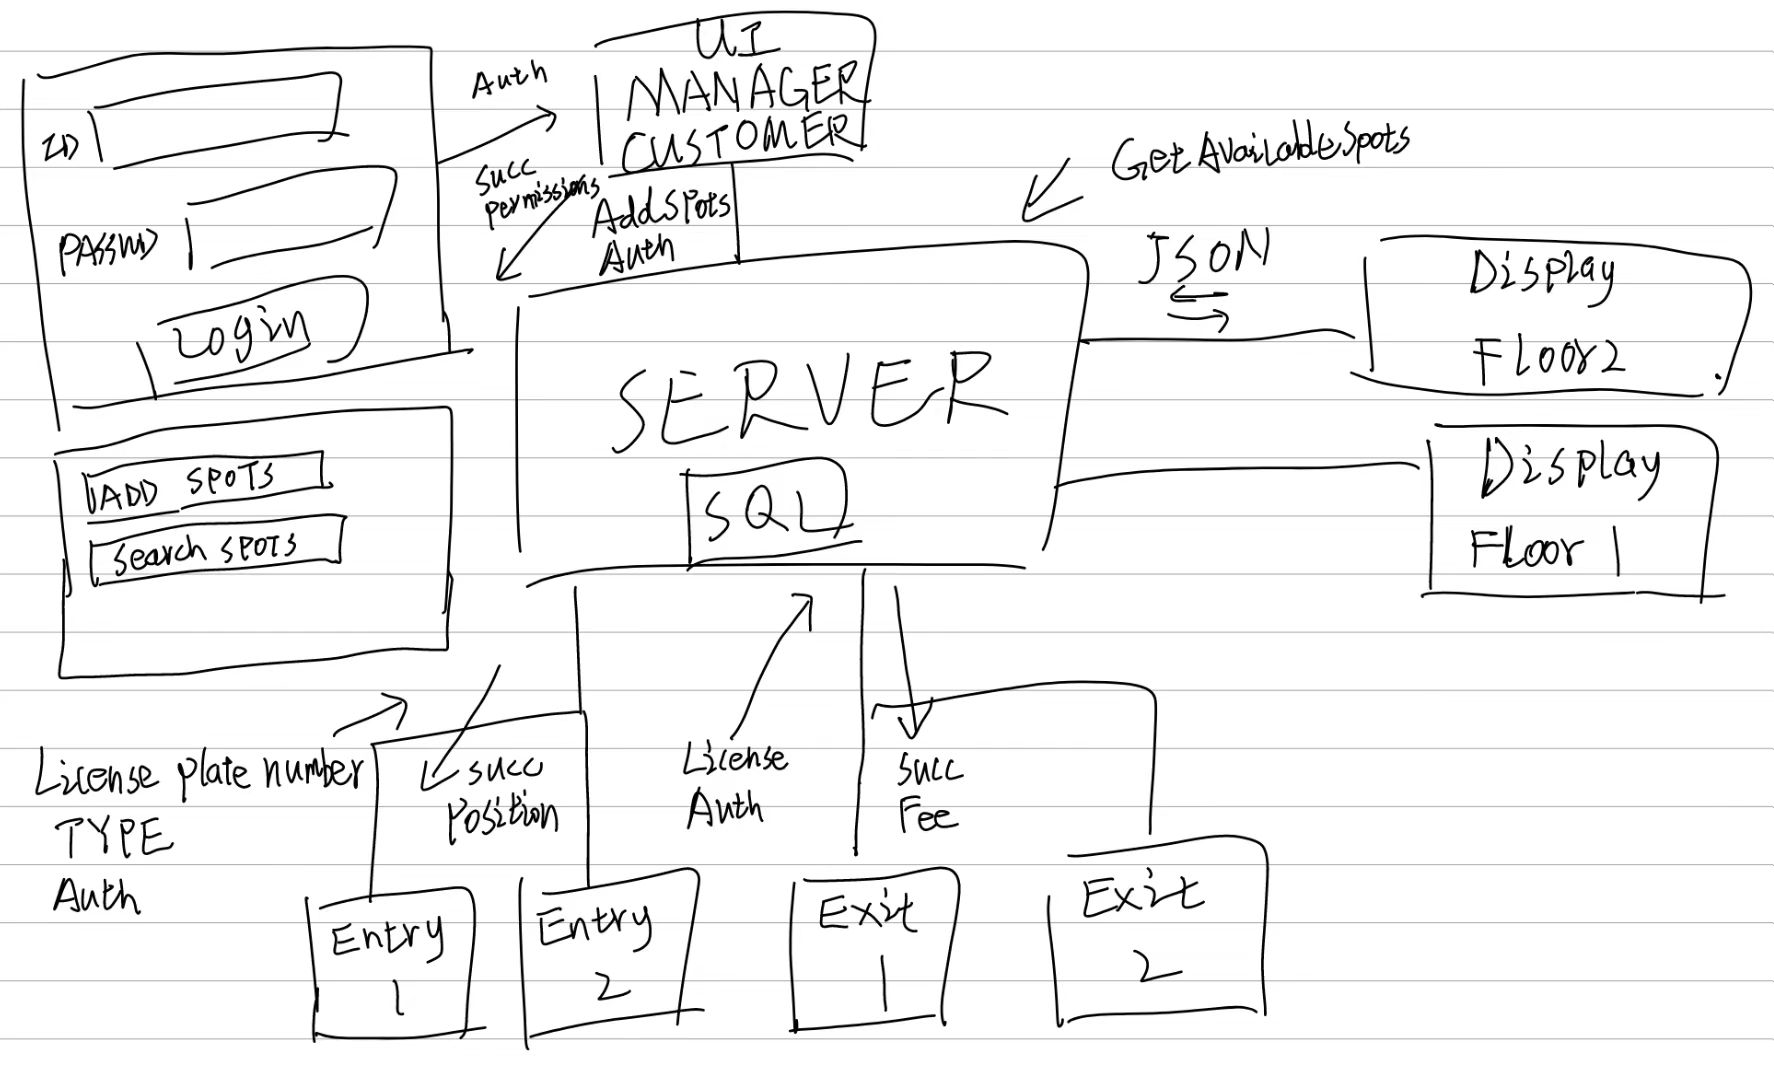
\includegraphics[width=0.8\textwidth]{pics/1.png}
			\captionof{figure}{Project Architecture}
		\end{center}
		
		The frontend of our project utilizes the Qt framework, a popular
		cross-platform application development framework. Qt provides a
		comprehensive set of tools and libraries for building graphical user
		interfaces (GUIs) efficiently. We leverage the Qt Designer tool to
		visually design the UI components, arrange layouts, and define their
		properties. Additionally, the Qt User Interface Compiler (uic) tool
		converts the UI design files into C++ code that can be seamlessly
		integrated with the backend logic. By leveraging the Qt toolchain, we
		can streamline the frontend development process, enhance code
		reusability, and achieve a consistent and visually appealing user
		interface across different platforms.
		\begin{center}
			\centering
			\includegraphics[width=0.8\textwidth]{pics/2.png}
			\captionof{figure}{Running on linux.}
		\end{center}
		
		\begin{center}
			\centering
			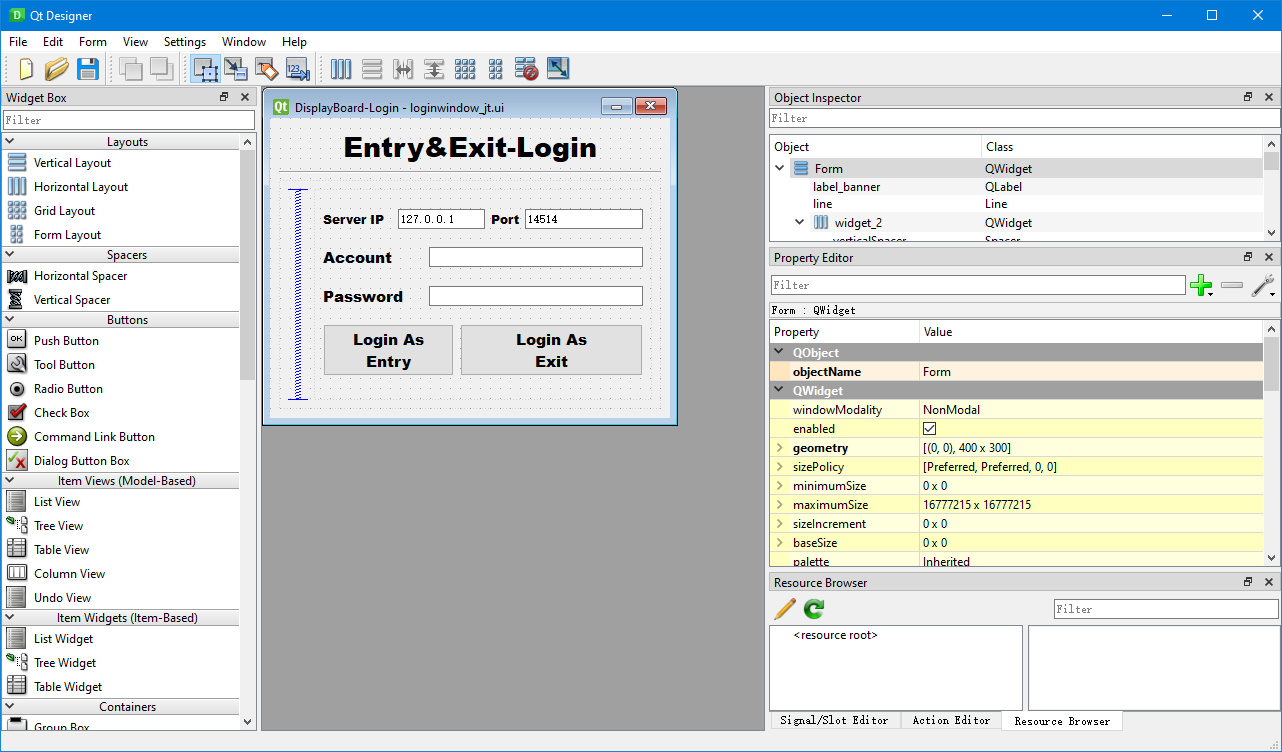
\includegraphics[width=0.8\textwidth]{pics/3.png}
			\captionof{figure}{Designer Page}
		\end{center}

		The communication between the frontend and backend of our project is
		facilitated using the TCP (Transmission Control Protocol) protocol. TCP
		provides a reliable and connection-oriented communication channel
		between the client (frontend) and server (backend). This ensures that
		data packets are delivered in order and without loss or corruption.
		
		To facilitate the exchange of data between the frontend and backend, we
		utilize the JSON (JavaScript Object Notation) format for serialization
		and transmission. JSON is a lightweight and widely supported data
		interchange format that allows for easy representation and parsing of
		structured data. By using JSON, we can effectively serialize complex
		data structures into a human-readable format that can be transmitted
		over the TCP connection, enabling seamless communication and data
		exchange between the frontend and backend components of our project.
		\begin{center}
			\centering
			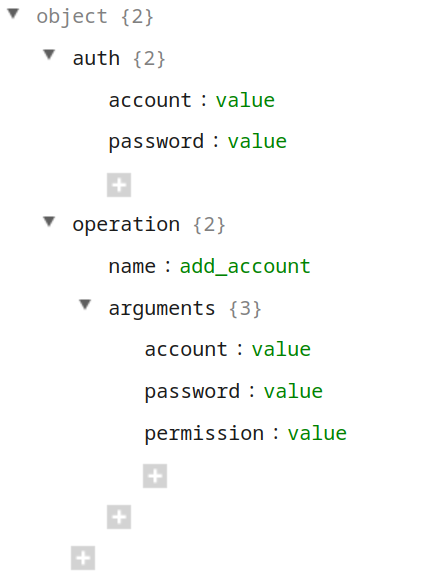
\includegraphics[width=0.7\textwidth]{pics/4.png}
			\captionof{figure}{JSON Data Example}
		\end{center}
	}
	\newpage
	\section{Management of source code and lifecycle by software tools(Git and Github)}
	%\subsection{git and github}
	{\slshape \selectfont 
		Version Control with Git:
		Git is a distributed version control system that enables efficient tracking and management of changes to the source code. Our team utilizes Git to maintain a central repository on GitHub, where all the source code files are stored and version controlled. 
		Git provides several advantages, including:\\
			\begin{itemize}
			\item [1)]
			Branching and Merging: Git allows us to create branches for different features, bug fixes, or experiments. This enables parallel development and easy merging of changes back into the main codebase.
			\item [2)]
			History and Rollback: With Git, we have a complete history of all changes made to the code. This facilitates easy identification of issues, bug tracking, and the ability to roll back to a previous state if necessary.
			\item [3)]
			Collaboration: Git enables seamless collaboration among team members. Each developer can work on their branch and merge changes with others, minimizing conflicts and ensuring efficient teamwork.
			\end{itemize}
			GitHub for Remote Repository:
			GitHub is a web-based hosting service for Git repositories which . Our team utilizes GitHub as the remote repository for our project. The benefits of using GitHub include:\\
			\begin{itemize}
			\item [1)]
			Centralized Repository: GitHub provides a centralized location for storing and managing our source code. It serves as a reliable backup and allows easy access to the code from anywhere.
			\item [2)]
			Collaboration and Code Review: GitHub offers features like pull requests and code review tools, which facilitate collaboration and maintain code quality. Team members can review each other's code, suggest improvements, and discuss changes before merging them into the main branch.
			\item [3)]		
			Issue Tracking: GitHub's issue tracking system allows us to create, assign, and track issues, bugs, and feature requests. This helps in effective project management and prioritization of tasks.
		\end{itemize}
	}
	\newpage
	\section{Testing}
	{\slshape \selectfont
		Testing is a crucial step in the development process. At the end of the
		testing, the code is delivered to the customer. It ensures that the
		software functions as intended, identifies any defects or issues, and
		verifies that the system meets the specified requirements. In the case
		of a frontend-backend separated project, testing becomes essential to
		ensure the seamless interaction between the UI and backend components.
		The testing process for our project involves separate unit testing for
		both the UI and the backend components, followed by integration testing
		to ensure their seamless interaction.
		
		We first tested each modular unit independently to ensure that the
		layout, appearance and behavior of the front-end UI elements matched
		the design, and that the back-end units performed the expected actions
		and produced the expected output correctly.
		
		After all the UI and backend components have undergone thorough unit
		testing, integration testing takes place. It verifies that the frontend
		and backend functionalities work together harmoniously, ensuring proper
		data exchange and preserving the desired system behavior.
		
		After testing, we merge the code from the dev branch to the main branch,
		indicating that the code has been accepted and moved from development to
		maintenance status.
		
	}
	\section{Bugs report}
	{\slshape \selectfont
		Our system uses the absolute coordinate to locate the UI which leads to its possible abnormally display.
	}
	\newpage
	\section{user manul}
	{\subsection{product character}
	\subsubsection{diversity and Searching}
	{\slshape \selectfont
		 This system allow administrator and customer to search for all unoccupied parking spots and it support multiple types of parking spots. There are spots for a specific type of vehicle, i.e., car, trunk, van, motorcycle etc.
	}
	\subsubsection{Fee for parking}
	{\slshape \selectfont
		The system support a per-hour parking fee model. For example, the first hour is free,
		and customers have to pay \$3 for the remaining hours, maximally \$50 per day.
	}
	\subsubsection{displaying board for free spot}
	{\slshape \selectfont
		Each parking floor has a display board showing any free spot for each spot type. Besides,if the parking is full, the system will show a message to the customer.
	}
	\newpage
	%经理的内容
	\subsection{For manager}
	\subsubsection{Searching}
	{\slshape \selectfont
		By entering account,password and floor, managers can easily get each floors information.
		\vspace{2cm}
		\begin{center}
			\centering
			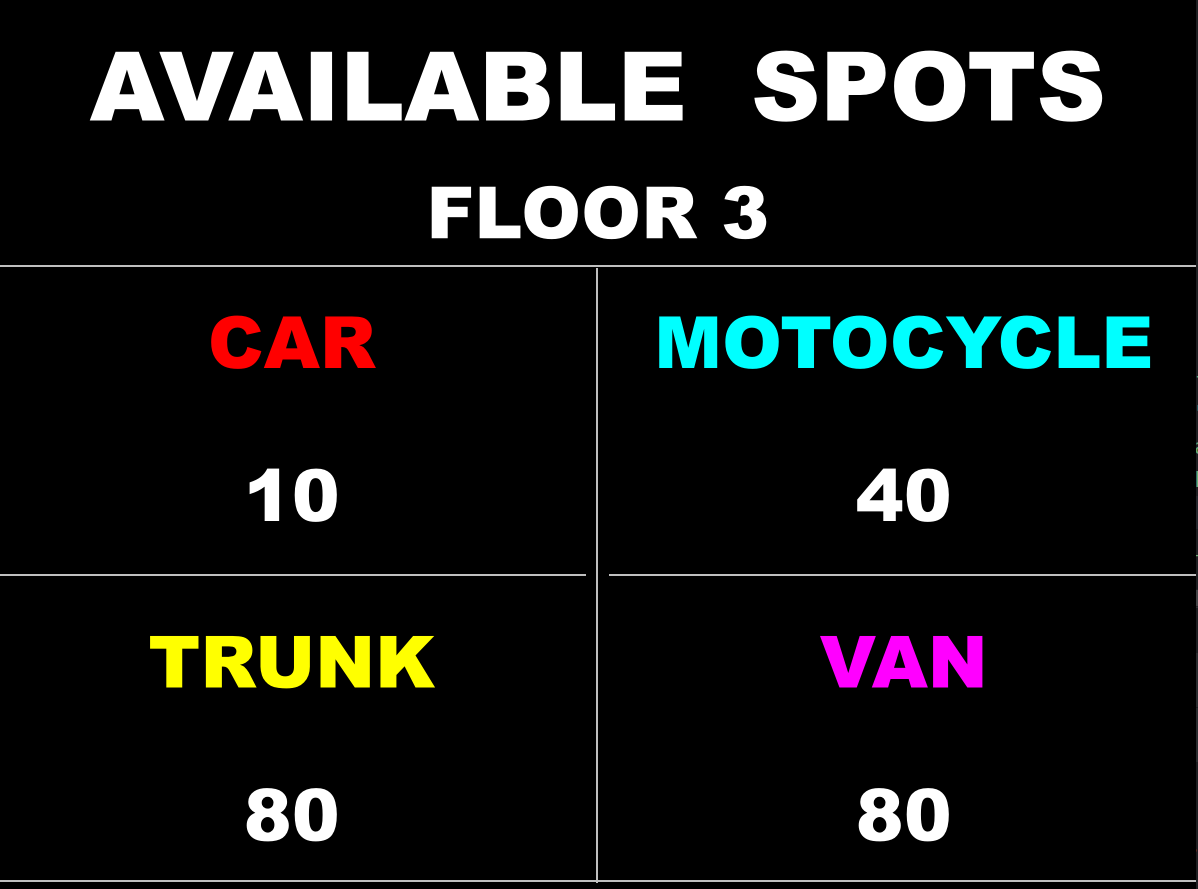
\includegraphics[width=0.6\textwidth]{pics/Floor3.png}
			\captionof{figure}{The informations of each floor}
		\end{center}
		\vspace{10cm}
		\subsubsection{Tools for editting spot}
		{\slshape \selectfont
			 The managers can browse, add, modify and delete spots and customer information
			\begin{center}
				\centering
				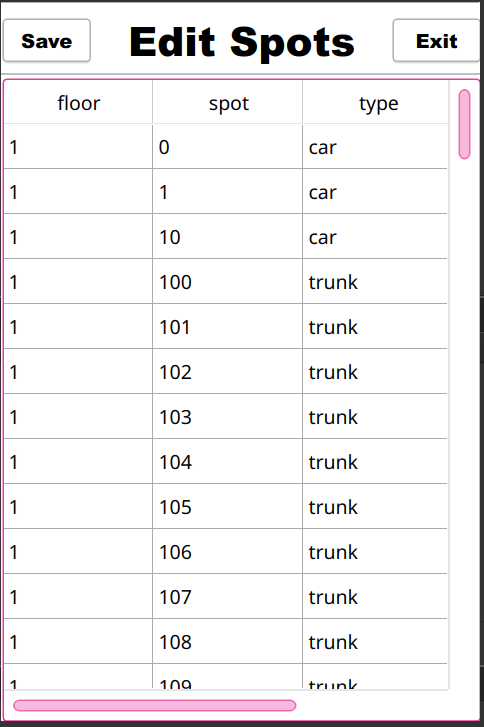
\includegraphics[width=0.4\textwidth]{pics/Edit.png}
				\captionof{figure}{The editor's UI}
			\end{center}
		}
		%\newpage
		\subsection{For customers}
		\subsubsection{Full Notice}
		{\slshape \selectfont
			 Customers will get a notice if the parking is full.
			And customers can get the information from the display board.
		}
		\newpage
		\subsubsection{paying}
		{\slshape \selectfont
			 When customers enter the park, they can choose the type of vehicle and enter the license plate number.
			\begin{center}
				\centering
				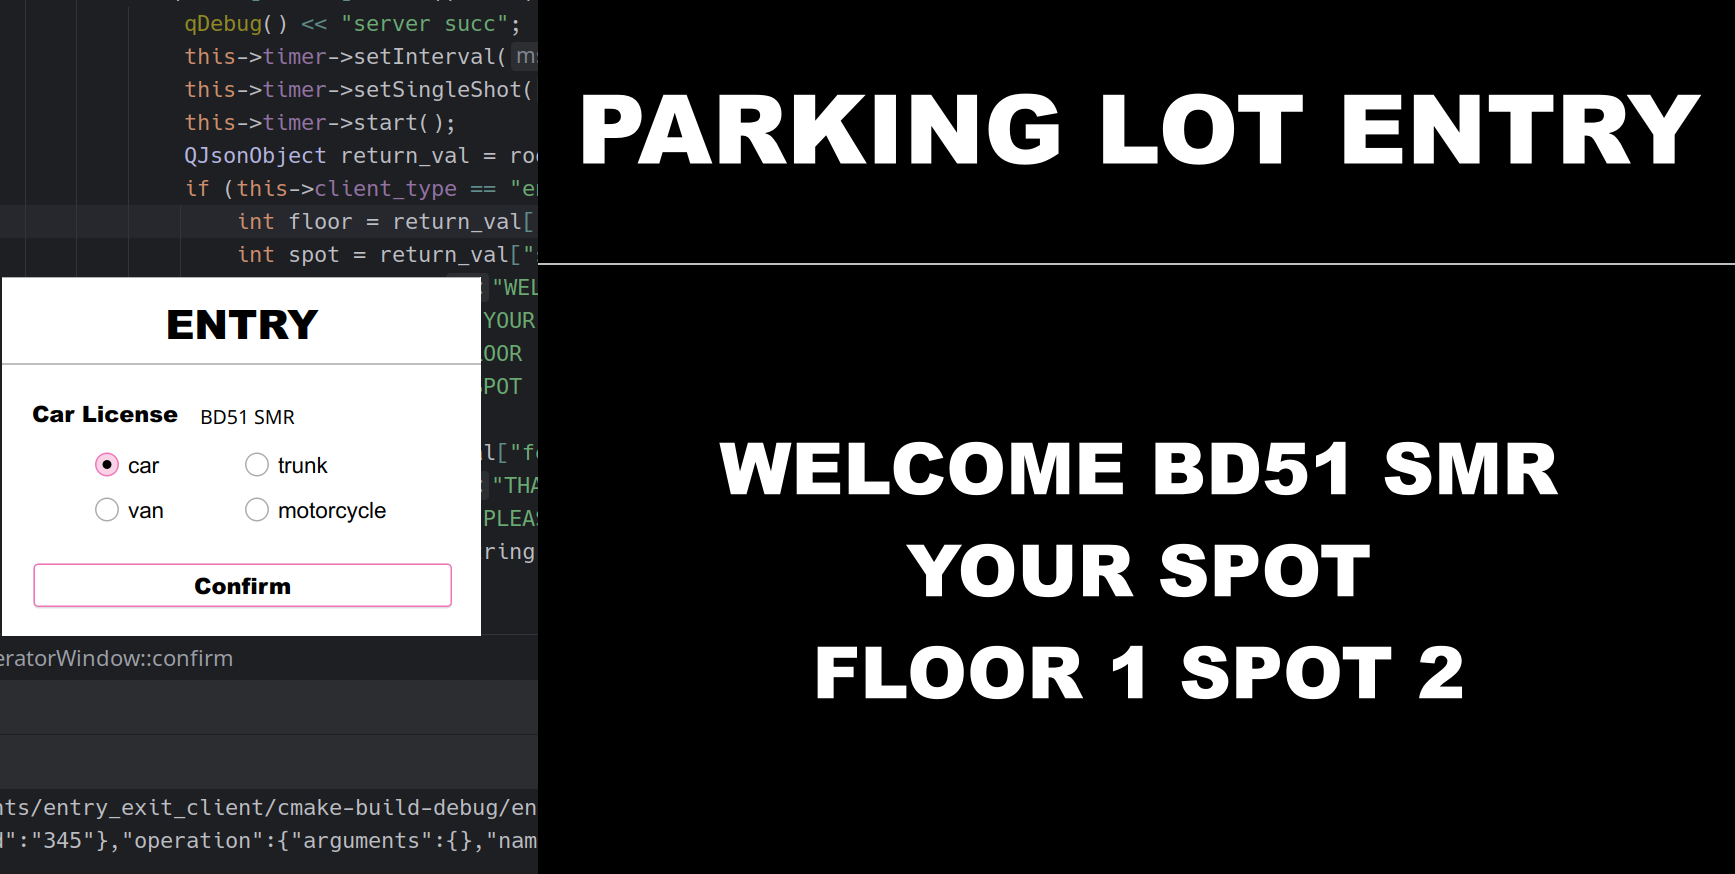
\includegraphics[width=0.7\textwidth]{pics/entry.png}
				\captionof{figure}{The entry UI}
			\end{center}
		
			Then if customers are going to exit the park, this system will calculate the bill and offer port to pay.
			\begin{center}
				\centering
				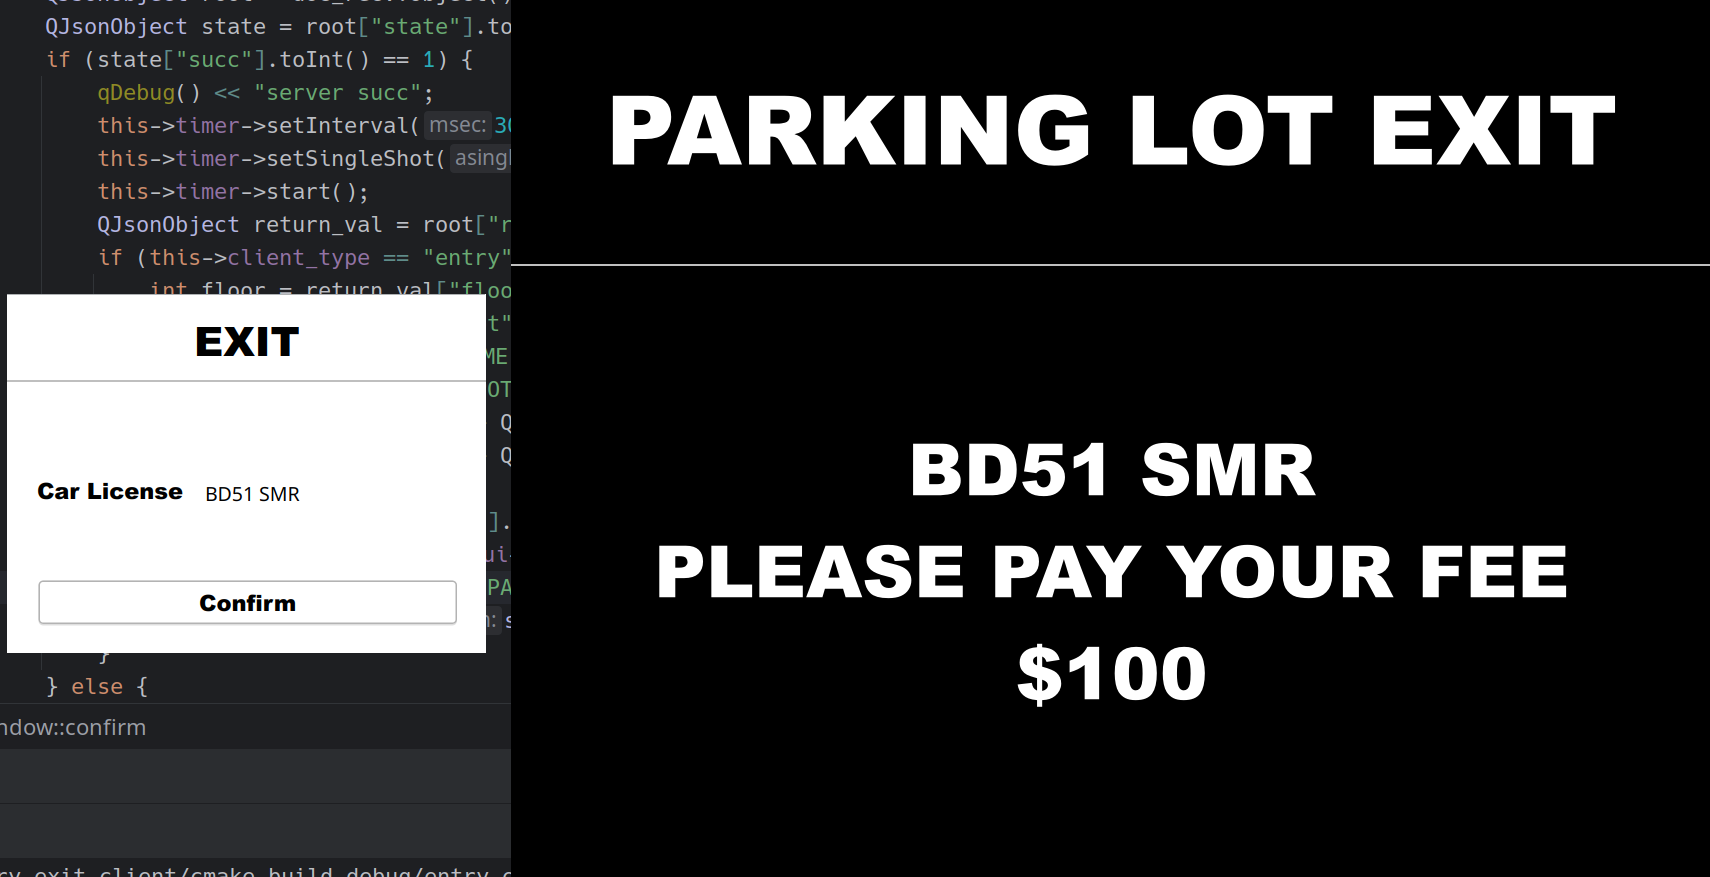
\includegraphics[width=0.6\textwidth]{pics/exit.png}
				\captionof{figure}{The exit UI}
			\end{center}
			
		}
		\subsubsection{Searching}
		{\slshape \selectfont
			By entering account,password and floor, customers can easily get each floors information.
			\begin{center}
				\centering
				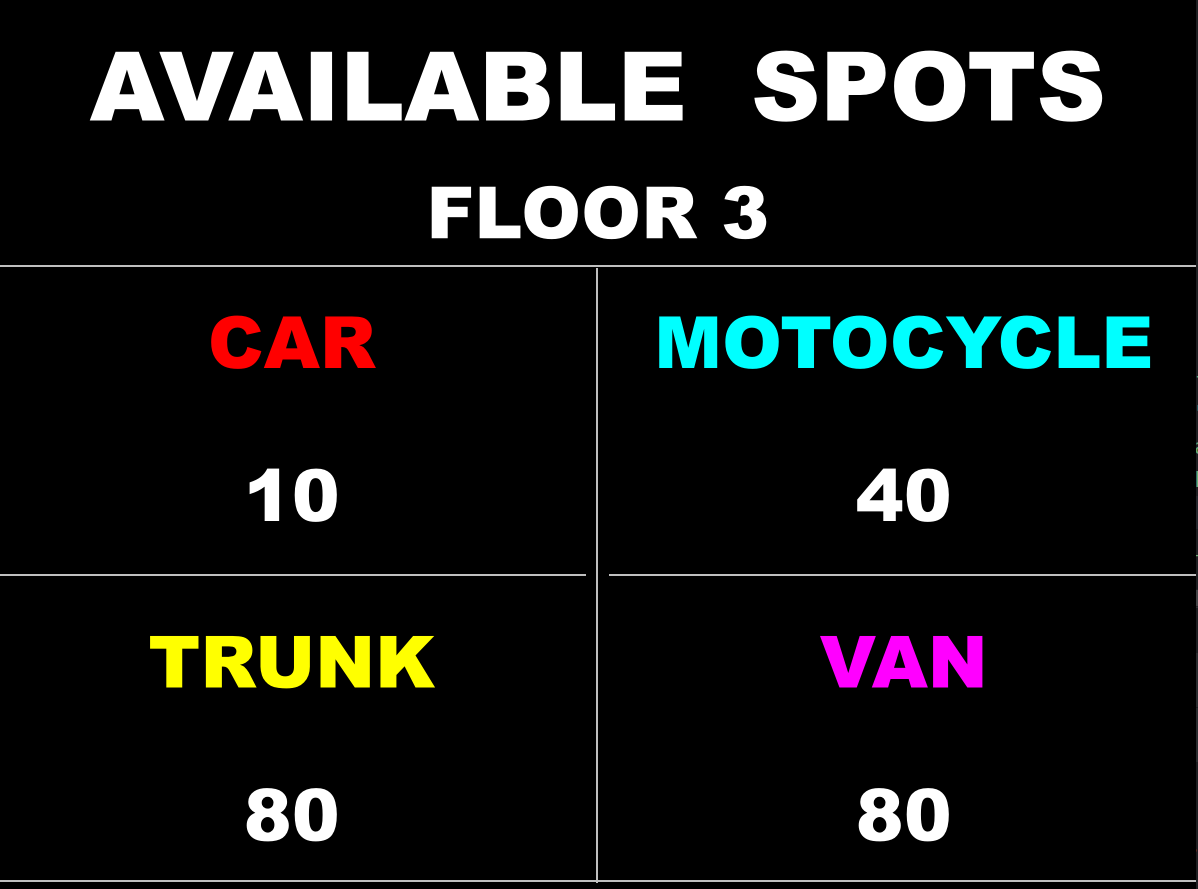
\includegraphics[width=0.4\textwidth]{pics/Floor3.png}
				\captionof{figure}{The informations of each floor}
			\end{center}
		}
	}
}	
